\documentclass[tikz]{standalone}
\usepackage{tikz}
\usepackage{amssymb}
\usetikzlibrary{positioning}
\usetikzlibrary{calc}
\usetikzlibrary{arrows,shapes,snakes,automata,petri}

\begin{document}
	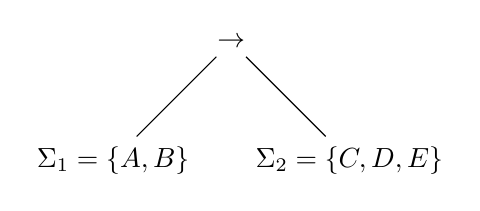
\begin{tikzpicture}[level distance=1.5cm,
	level 1/.style={sibling distance=3cm},
	level 2/.style={sibling distance=1.25cm},
	level 3/.style={sibling distance=0.625cm}]
	\node{$\rightarrow$}
		child{node{$\Sigma_1=\{A,B\}$}
			%child{node{A}}
			%child{node{B}}
		}
		child{node{$\Sigma_2=\{C,D,E\}$}
			%child{node{$\circlearrowleft$}
			%	child{node{C}}
			%	child{node{D}}
			%}	
			%child{node{E}}
		};
	\end{tikzpicture}
\end{document}